% \subsection{Boundary Conditions, work and energy, conductors}
\subsection{Electric Potential}
	\subsubsection{Introduction}
		\label{subsubsec:electricpotential intro}
		The electric field $\vb E$ is not just \textit{any} old vector function. It is 
		a special kind of vector function, one whose curl is zero. $\vb E = y\vu x$, for 
		example, could not possibly be an electrostatic field. No set of charges, regardless
		of their sizes and positions, could ever produce such a field. 

		We're going to exploit this special property of electric fields to reduce a vector
		problem (finding $\vb{E}$), to a much simpler \textit{scalar} problem. Theorem \ref{thm:irrotational-fields}
		states that any vector field whose curl is zero is equal to the gradient of some scalar
		field. What we are going to do now amounts to a proof of such claim, in the context
		of electrostatics.

		Because $\curl\vb{E}=\vb{0}$, the line integral of $\vb E$ around any closed loop is
		zero.\footnote{From Stokes' Theorem} Because $\displaystyle \oint \vb{E}\cdot\dd{\vb*{\ell}}=0$,
		the line integral of $\vb E$ from a point $\vb a$ to point $\vb b$, is the same for all paths\footnote{otherwise you could go \textit{out} along a path $a$ and return
		along a path $b$, and obtain $\oint\vb{E}\cdot\dd{\vb*{\ell}}\neq0$}. Because the line integral
		is independent of path, we can define a function
		\begin{equation}\label{eq:E_linepath}
			V(\vb{r}) \equiv -\int_{\mathcal{O}}^{\vb{r}} \vb{E}\cdot\dd{\vb*{\ell}}
		\end{equation}
		Here, $\mathcal{O}$ is some standard reference point on which we have agreed to 
		beforehand. $V$ then depends only on the point $\vb r$. It is called the \textbf{Electric potential}.

		The potential \textit{difference} between two points $\vb a$ and $\vb b$ is:
		\begin{align*}
		    V(\vb b) - V(\vb a) 
			&= 
			-\int_{\mathcal{O}}^{\vb{b}} \vb{E}\cdot\dd{\vb*{\ell}} 
			+\int_{\mathcal{O}}^{\vb{a}} \vb{E}\cdot\dd{\vb*{\ell}} \\
			&= 
			-\int_{\mathcal{O}}^{\vb{b}} \vb{E}\cdot\dd{\vb*{\ell}} 
			-\int^{\mathcal{O}}_{\vb{a}} \vb{E}\cdot\dd{\vb*{\ell}} \\
			&= 
			-\int_{\vb{a}}^{\vb{b}} \vb{E}\cdot\dd{\vb*{\ell}} 
		\end{align*}
		Now, the fundamental theorem for gradients state that
		\begin{equation}
			V(\vb b) - V(\vb a) = \int_{\vb a}^{\vb b} (\grad V)\cdot \dd{\vb*{\ell}}
		\end{equation}
		so,
		\begin{equation}
			\int_{\vb a}^{\vb b} (\grad V)\cdot \dd{\vb*{\ell}}
			=
			-\int_{\vb{a}}^{\vb{b}} \vb{E}\cdot\dd{\vb*{\ell}} 
		\end{equation}
		Since, finally, this is true for any points $\vb{a}$ and $\vb{b}$, the 
		integrands must be equal. Hence:
		\begin{theorem}{Electric fields come from scalar potentials}
			\begin{equation}\label{eq:E_potential}
		       \vb{E} = -\grad V
			\end{equation} 
		\end{theorem}
		Equation (\ref{eq:E_potential}) is the differential version of (\ref{eq:E_linepath});
		it says that the electric field is the gradient of a scalar potential, which we set out
		to prove.

		Notice the subtle but crucial role played by the path independence (or equivalently,
		the fact that $\curl\vb{E}=\vb{0}$) in this argument. If the line integral of $\vb E$
		depended on the path taken, then the definition of $V$ (\ref{eq:E_potential}), would become nonsense.
		It simply would not define a function, since changing the path would alter the value of 
		$V(\vb r)$. 
		
	\subsubsection{Some comments on Potentials}
		\subsubsubsection{The name}
			The word ``potential'' is sort of a misnomer, because it reminds you of the concept
			of potential \textit{energy}. While there is a connection between the two, that
			is not precisely what electric potential means, and they are completely different terms.
			Although, the name potential here comes from the fact that taking the gradient
			results in a force, which is analogous to gravitational potential $\Phi$,
			\[
				\vb{F} = -\grad\Phi,
			\]
			and in fact all kinds of other \textit{potentials} used in other physics terms. Hence, for this reference, the name potential is appropriate.
			Incidentally, a surface over which the potential is constant is called an \textbf{equipotential}
		\subsubsubsection{Advantage of the potential formula}
			Knowledge of the potential field $V$ immediately means that you can get $\vb E$, just by takign the gradient $\vb E = -\grad V$.
			This is quite fascinating, since $\vb E$ is a vector quantity of three components, while $V$ is simply a scalar of one
			component. As such, the possibility that one function contains all the information of three independent functions is
			quite absurd. However, the answer is that the three components of $\vb E$ are not really quite independent.
			They are, in fact, explicitly related by the condition we used to prove the potential, and that is $\curl\vb E = \vb{0}$

			In terms of components, they can be expressed as
			\begin{align*}
				\pdv{E_x}{y}=\pdv{E_y}{x}&&
				\pdv{E_z}{y}=\pdv{E_y}{z}&&
				\pdv{E_x}{z}=\pdv{E_z}{x}
			\end{align*}

			As such, the components of $\vb E$ are really coupled differential equations that relate to each other.
			This brings us back to our observation in the beginning, $\vb E$ is a \textit{special kind} of vector field,
			and the potential formulation exploits these feauture to a maximun advantage, reducing a vector problem to
			a scalar one, where there is no need to inconvenience ourselves with components.
		\subsubsubsection{The arbitrary reference point}
			The choice for an arbitrary reference point $\mathcal{O}$ seems quite strange. However, here,
			we argue that the electric potential is inherently defined only up to an arbitrary additive constant,
			because the choice of reference point $\mathcal O$ is arbitrary. If the reference point is changed from, say
			$\mathcal O$ to $\mathcal{O}'$, then
			\begin{align*}
				V'(r) 
				&= -\int_{\mathcal{O}'}^{\vb r} \vb{E} \cdot \dd{\vb*{\ell}}\\
				&= -\int_{\mathcal{O}}^{\vb r} \vb{E} \cdot \dd{\vb*{\ell}}
				   -\int_{\mathcal{O}'}^{\mathcal{O}} \vb{E} \cdot \dd{\vb*{\ell}}\\
				&= V(\vb r) + K
			\end{align*}
			where $K$ is a constant independent of $\vb r$. Consequently, 
			\[
				V'(\vb b) - V'(\vb a) = V(\vb b) - V(\vb a)
			\]
			and as such, potential differences are physically meaningful, while the absolute 
			value of the potential is not. Since $V'(\vb r)$ is only $V(\vb r)+K$, then
			\[
				\grad V' = \grad V
			\]
			and as such the electric field is likewise unchanged even though the absolute potential
			is different. The choice of reference point is therefore mostly a matter of convenience.
			One can choose $V=0$ at any convenient location, much like choosing where to define zero
			altitude. What matters physically is the difference in potential between two points. Therefore,
			saying a point has a particular \textit{absolute} potential has no intrinsic meaning unless
			a reference has been specified.
			
			As such, there is no physically privileged zero of electric potential, and one may
			choose the reference point wherever convenient, because changing it does not alter
			the potential difference nor the vector field that arises from the potential.

			There is, however, a particularly convenient convention in electrostatics: take the potential
			to vanish at infinity, i.e.,
			\[
				V(\infty)= 0
			\]
			Ordinarily, then, we ``set the zero of potential at infinity''. Since $V(\mathcal{O})=0$, choosing a reference
			point is equivalent to selecting a place where $V$ is to be zero). This works naturally for 
			localized charge distributions because the electric field becomes 
			negligible sufficiently far away. For an infinite plane of charge, however, this convention 
			fails: the potential does not approach a finite value at infinity. For example,	
			\[
				V(z) = -\int_\infty^z \frac{\sigma}{2\varepsilon_0}\dd{z} = -\frac{\sigma}{2\varepsilon_0}(z-\infty)
			\]
			The potential in this case is not finite. 
			The remedy is simply to choose some other reference point. However, this problem is merely theoretical. 
			In practice, there is no electric potential that extends infinitely, and one can always define a point
			be $V=0$. 
		\subsubsubsection{Potentials obey superposition}
			The original superposition principle pertains to the force acting on some test 
			charge $q$. It says that the total force acting on $q$ is the vector sum of all
			the forces attributable to the source charges individually.
			\[
				\vb{F} = \vb{F}_1 + \vb{F}_2 + \cdots
			\]
			Dividing by $q$, we see that the electric field also obeys the principle of superposition.
			\[
				\vb{E} = \vb{E}_1 + \vb{E}_2 + \cdots
			\]
			If we integrate from the common reference point to $\vb r$, it follows that the 
			potential also satisfies such principle
			\[
				V = V_1 + V_2 + \cdots
			\]
			Therefore, the potential at any given point is the sum of the potentials due to
			all the charges separately. Only this time, the quantity is an ordinary sum, not 
			a vector sum, which makes it more convenient and easier to work with.
		\subsubsubsection{Units of Potential}
			In the customary \textit{Syst\`eme International} (SI) units, force is measured in
			newtons and charge in coulombs, and as such, electric fields are measured in newtons per 
			coulomb. Accordingly, potentials are measured in newton-meters per coulomb.

			A joule per coulomb is called a \textbf{volt}
			\[
				\SI{1}{V} = 1 \frac{\unit{Nm}}{\unit{C}} 
			\]
	\subsubsection{Poisson's and Laplace's Equation}
		We found in \S \ref{subsubsec:electricpotential intro} that the electric field 
		can be written as the gradient of a scalar potential
		\[
			\vb{E} = -\grad V
		\]
		The question then arises: What do the divergence and curl of  the electrice field $\vb E$,
		$\div\vb E = \rho/\varepsilon_0$ and $\curl\vb E = \vb{0}$, look like in terms
		of $V$? Well, we have
		\begin{align*}
			\vb{E} &= -\grad V\\
			\div\vb{E} &= \div(-\grad V)\\
			\div\vb{E} &= -\lpc V
		\end{align*}

		And so, apart from the persistent minus sign, the divergence of $\vb E$ is the 
		Laplacian of $V$. Gauss's Law, then, says that
		\begin{theorem}{Poisson's Equation}
			\begin{equation}\label{eq:poisson_theorem}
				\lpc V = -\frac{\rho}{\epsz} 
			\end{equation}	
		\end{theorem}
		This is known as \textbf{Poisson's equation}. In regions where there are no charge, so
		$\rho=0$, Poisson's equation reduces to \textbf{Laplace's equation}
		\begin{theorem}{Laplace's Equation}
		    \begin{equation}
		        \lpc V = 0
		    \end{equation}
		\end{theorem}
		For the curl, we have
		\[
			\curl\vb E = \curl(-\grad V) = \vb{0}
		\]
		But that is no condition on $V$. The curl of a gradient is \textit{always} zero. 
		In fact, we used the curl law to show that $\vb E$ could be expressed as a gradient
		of a scalar, so it's not really surprising that this is the case. $\curl\vb E = \vb{0}$
		\textit{permits} $\vb E = -\grad V$, and in return, $\vb E = -\grad V$ \textit{guarantees}
		$\curl\vb E = \vb{0}$. It only takes one differential equation, Poisson's equation,
		to determine $V$, because $V$ is a scalar. For $\vb E$, we needed two, the divergence 
		and the curl. 

		In this case, then, we can say that $\lpc V = - \dfrac{\rho}{\epsz}$ is the 
		\textbf{\textit{field equation}} governing electrostatics.
		
	\subsubsection{The Potential of a Localized Charge Distribution}
		We defined $V$ in terms of $\vb E$, and found that it is more convenient to do so since
		it makes calculations significantly easier. Normally, though, it's $\vb E$ that we are looking
		for (if we already knew $\vb E$, there wouldn't be much point in calculating $V$). The idea is that
		it might be easier to get $V$ first, and then calculate $\vb E$ by taking the gradient. Typically, then,
		we know where the charge is (i.e, we know $\rho$), and we want to find $V$. Poisson's equation
		relates $V$ and $\rho$, but unfortunately, it is formulated in such a way that it provides $\rho$
		given that we already knew $V$, whereas we want to know $V$, knowing $\rho$. What we must do then, is 
		``invert'' Poisson's equation. For this section, that is the task which we set out to do. However,
		 we shall do it by roundabout means, beginning, as usual, with a point charge at the origin.

		 The electric field is
		 \[
			 \vb{E} = \frac{1}{4\pi\epsz} \frac{1}{r^2}\vu{r}  
		 \]
		 and the line element is
		 \[
			 \dd{\vb* \ell} = \dd{r}\vu{r} + r\dd{\theta}\vu*{\theta} + r\sin\theta\dd{\phi}\vu*{\phi}
		 \]
		 Hence, we have
		 \[
			 \vb{E}\cdot \dd{\vb* \ell} = \frac{1}{4\pi\epsz} \frac{q}{r^2} \dd{r}
		 \]
		 Setting the reference point at infinity, the potential of the point charge $q$ at the origin is
		 \begin{align*}
		     V(r) 
			 &=
			 -\int_{\mathcal{O}}^{r}\vb{E}\cdot \dd{\vb* \ell}\\
			 &=
			 -\frac{1}{4\pi\epsz} \int_{\infty}^r \frac{q}{r'^2}\dd{r'} \\
			 &=
			 \frac{1}{4\pi\epsz}\eval{\frac{q}{r'}}^r_\infty\\
			 &=
			 \frac{1}{4\pi\epsz} \frac{q}{r} 
		 \end{align*}
		 We see here the advantage of using infinity as a reference point; it kills the lower limit
		 of the integral. Notice the sign of $V$; presumably, the conventional minus sign in the definition (\ref{eq:poisson_theorem})
		 was chosen in order to make the potential of a positive charge come out positive. It is useful to remember that regions og positive
		 charge are potential `hills', whereas regions of negative charge are potential	`valleys', and the electric field always points
		\textit{downhill} from the high point of the potential to the low point.
		
		In general, the potential of a point charge $q$ is
		\begin{equation}
		   V(\vb x) = \frac{1}{4\pi\epsz} \frac{q}{r}   
		\end{equation}
		where $r$ is the distance from $q$ to a point $\vb x$\footnote{Forgive the change of variables, the text becomes confusing so this is to help me}.
		i.e., $\vb r = \vb{x} - \vb{x}_q$, where $\vb{x}_q$ is the position of $q$. Invoking the superposition principle, then, we find that the potential
		of a collection of charges is 
		\begin{equation}
		    V(\vb x) = \frac{1}{4\pi\epsz} \sum_i \frac{q}{r_i},
		\end{equation}
		or, for a continuous distribution,
		\begin{equation}
			V(\vb x) = \frac{1}{4\pi\epsz}\int \frac{1}{r} \dd{q}
		\end{equation}
		In particular, for a volume charge, it is,
		\begin{theorem}{Potential for a charge distribution}
			\begin{equation}\label{eq:charge_potential}
				V(\vb x) = \frac{1}{4\pi\epsz}\int \frac{\rho(\vb x')}{r}\dd{V}  
			\end{equation}
		\end{theorem}
		
		Here, $\vb x'$ denotes the test point being integrated over all $\R^3$ in the integral. 
		This is the equation we were looking for, which tells us how to compute $V$ when we know
		$\rho$. It is, if you will, the \textit{solution} to Poisson's equation, for a localized charge
		distribution. Compare this to the corresponding equation for the electric field:
		\begin{equation}
			\vb{E}(\vb x) = \frac{1}{4\pi\epsz} \int \frac{\rho(\vb x')}{r^2} \vu{r} \dd{V}
		\end{equation}
		The main point here is that the pesky unit vector $\vu{r}$ is gone, so there is no need to
		fuss with components. Here, we go back to denoting general position to $\vb r$, since it is an 
		arbitrary point and may be relabeled.. The potentials of line and surface charges are
		\begin{equation}
			V(\vb r) = \frac{1}{4\pi\epsz}\int \frac{\lambda(\vb r')}{r^2}\dd{\ell}  
		\end{equation}
		and
		\begin{equation}
			V(\vb r) = \frac{1}{4\pi\epsz}\int \frac{\sigma(\vb r')}{r^2}\dd{S}  
		\end{equation}
		We warn you, however, that everything presented in this section is predicated upon the assumption
		that the reference point is at infinity. This is hardly apparent from (\ref{eq:charge_potential}),
		but remember that we \textit{got} that equation of the potential from a point charge at the origin, which
		is only valid when $\mathcal{O} = \infty$. If one tries to apply these formulae to one of those 
		artificial problems where the charge itself extends to infinity, the integral will diverge.

	\subsubsection{Boundary Conditions}
		
		In the typical electrostatic problem, one is given a source charge distribution
		$\rho$, and is tasked to fined the electric field $\vb E$ it produces. Unless the
		symmetry of the problem allows a solution by Gauss's law, it is generally in one's 
		advantage to calculate the potential first, as an intermediate step. These are the 
		three fundamental quantities in electrostatics are: $\rho, \vb{E}$, and $V$. We have,
		in the course of the discussion, derived most of the formulae interrelating them.
		We began with just two experimental observations: (1) the principle of superposition%
		--a broad general rule applying to \textit{all} electromagnetic forces, and 
		(2) Coulomb's law--the fundamental law of electrostatics. From these, all else
		followed.

		One may notice, while testing out these problems, that the electric field always 
		undergoes a discontinuity when crossing a surface charge $\sigma$. It is, in fact,
		a simple matter to find the \textit{amount} by which $\vb E$ changes at such a boundary.
		Suppose we draw a wafer-thin Gaussian pillbox, extending just barely over the edge
		in each direction (Fig. \ref{fig:pillbox}), Gauss's law says that
		\[
			\oint_S \vb{E}\cdot\dd{\vb S} 
			= 
			\frac{1}{\epsz}Q_\text{enc} 
			= 
			\frac{1}{\epsz} \sigma A 
		\]
		where $A$ is the area of the pillbox lid (If $\sigma$ varies from point to point
		or the surface is curved, we must pick $A$ to be extremely small.) Now, the \textit{sides}
		of the pillbox contribute nothing to the flux. In the limit, as the thickness $\varepsilon$
		goes to zero, so we are left with
		\begin{equation}
			E_{\text{above}}^\perp - 
			E_{\text{below}}^\perp - 
			= \frac{1}{\epsz}\sigma 
		\end{equation}
		where $E_\text{aboce}^\perp$ denotes the component of $\vb E$ that is perpendicular
		to the surface immediately above, and $E_\text{below}$ is the same, only below the surface.
		For consistency, we let \textit{upward} be the positive direction for both. 
		
		A conclusion we can form is that the normal component of $\vb E$ is discontinuos by 
		an amount $\sigma/\epsz$ at any boundary. In particular, when there is \textit{no} surface
		charge, $E^\perp$ is continuous, as for instance, at at the surface of a uniformly
		charged solid sphere.

		\begin{figure}[h]
			\centering
			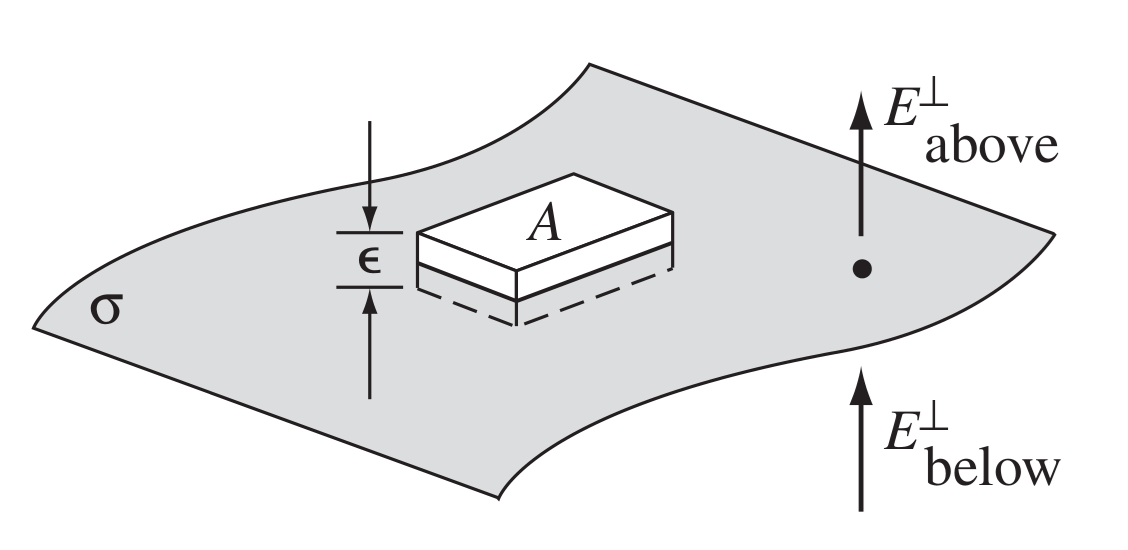
\includegraphics[width=2in]{images/waferthin.png}
			\caption{The setup of the Gaussian pillbox problem}
			\label{fig:pillbox}
		\end{figure}
		The \textit{tangential} component of $\vb E$, by contrast, is \textit{always} continuous.
		For if we apply Eq. \ref{eq:ointEdl=0},
		\begin{equation}
			\oint \vb{E}\cdot\dd{\vb* \ell} = 0
		\end{equation}
		to the thin rectangular loop of Fig. {\color{red}TBA}, the ends give nothing (as $\varepsilon\to0$), and 
		both sides give $E^\parallel_\text{above}l - E_\text{below}^\parallel l$, so
		\begin{equation}
			\vb{E}^\parallel_\text{above}
			=
			\vb{E}^\parallel_\text{below}
		\end{equation}
		where $\vb{E}^\parallel$ stands for the components of $\vb E$ \textit{parallel} to
		the surface. The boundary conditions on $\vb E$, Fig. {\color{red}TBA} and Fig. {\color{red}TBA},
		can be combined into a single formula:
		\begin{equation}
			\label{eq:Eabove-Ebelow=vnu}
			\vb{E}_\text{above} - \vb{E}_{below} = \frac{\sigma}{\epsz} \vu{n}
		\end{equation}
		where $\vu n$ is a unit vector perpendicular to the surface, pointing from \textit{below}
		to \textit{above}.

		The potential, meanwile, is continuos across \textit{any} boundary (Fig. {\color{red}TBA}),
		since
		\begin{equation}
			V_\text{above}
			-
			V_\text{below}
			=
			-\int^{\vb{b}}_{\vb{a}} \vb{E}\cdot\dd{\vb* \ell} 
		\end{equation}
		as the path length shrinks to zero, so too does the integral:
		\begin{equation}
			V_\text{above}
			=
			V_\text{below}
		\end{equation}
		However, the \textit{gradient} of $V$ inherits the discontinuity $\vb E$; since 
		$\vb E = -\grad V$. Eq. \ref{eq:Eabove-Ebelow=vnu} implies that
		\begin{equation}
			\grad V_\text{above}
			- \grad V_{below}
			= 
			-\frac{\sigma}{\epsz} \vu{n}
		\end{equation}
		or, mroe conveniently,
		\begin{equation}
			\pdv{V_\text{above}}{n} 
			- \pdv{V_\text{below}}{n} 
			= 
			-\frac{\sigma}{\epsz} 
			\label{eq:normderiv=-sigman}
		\end{equation}
		where
		\begin{equation}
			\pdv{V}{n} = \grad V\cdot \vu{n} 
		\end{equation}
		denotes the \textbf{normal derivative} of $V$, i.e., the rate of change in the direction
		perpendicular to the surface.

		Note that these boundary conditions relate the fields and potentials \textit{just}
		above and \textit{just} below the surface. For example, the derivatives in (\ref{eq:normderiv=-sigman})
		are the \textit{limiting} values as we approach the surface from either side.

	\newpage
\subsection{Work and Energy}
	\subsubsection{The Work it takes to Move a Charge}
		Suppose you have a stationary configuration of source changes, and you want to move
		a test charge $Q$ from point $\vb a$ to point $\vb b$. A question can be raised: 
		How much work will you have to do? At any point along the path, the electric force
		on $Q$ is $\vb F = Q\vb E$. The force \textit{you} must exert, in opposition to this
		electrical force, is $-Q \vb{E}$. The work done is therefore
		\begin{align*}
		    W
			&=
			\int_{\vb{a}}^{\vb{b}} \vb{F}\cdot\dd{\vb* \ell}\\
			&=
			-Q \int_{\vb{a}}^{\vb{b}} \vb{E}\cdot\dd{\vb* \ell}\\
			&=
			Q\bqty{V( \vb{b}) - V \vb{a}}
		\end{align*}

		Notice that the answer is indepenent of the path you take from $\vb a$ to $\vb b$;
		in mechanics, then, we would call the electrostatic force \textit{conservative}. Dividing
		through by $Q$, we have
		\begin{equation}
		    V( \vb{b} ) - V( \vb{a} )
			=
			\frac{W}{Q} 
		\end{equation}

		In other words, the potential difference between points $\vb a$ and $\vb b$ is equal
		to the work for unit charge required to carry a particle from $\vb a$ to $\vb b$. In
		particular, if you want to bring $Q$ in from far away and stick it at a point $\vb r$,
		the work you must do is
		\[
			W = Q\bqty{
				V( \vb{r} ) - V(\infty)
			}
		\]
		and so, if you have set the referece point at infinity, the work done is
		\begin{theorem}{Work done in an electric potential}
			\begin{equation}
				\label{eq:workcharge}
				W = QV( \vb{r} )
			\end{equation}
		\end{theorem}

		In that sense, \textit{potential} is the potential \textit{energy} (the work it takes
		to create the system) \textit{per unit charge} (just as the \textit{field} is the
		\textit{force} per unit charge).
	\subsubsection{The Energy of a Point Charge Distribution}
		How much work would it take to assemble an entire \textit{collection} of point charges?
		Imagine bringing in the charges, one by one, from far away. The first charge $q_1$,
		takes \textit{no} work, since there is no field yet to fight against. Now, we bring
		in $q_2$. Acording to
		(\ref{eq:workcharge}),
		this will cost $q_1V_1(\vb{r}_2)$, where $V_1$ is the potential due to $q_1$, and
		$\vb{r}_2$ is the place that we're  putting $q_2$:
		\[
			W_2
			=
			\frac{1}{4\pi\epsz}
			q_2\pqty{
				\frac{q_1}{r_{12}} 
			}
		\]
		where $r_{12}$ is the distance between $q_1$ and $q_2$ once they are position. As 
		you bring in each charge, pin it down to its final location, so that it does not move
		when you bring the next charge. Now, we bring $q_3$, this requires work $q_3 V_{1,2}(\vb{r}_3)$,
		where $V_{1,2}$ is the potential due to charges $q_1$ and $q_2$. Thus
		\[
			W_3 = 
			\frac{1}{4\pi\epsz}
			q_3\pqty{
				\frac{q_1}{r_{13}} 
				+
				\frac{q_2}{r_{23}} 
			}
		\]
		Similarly, the extra work to bring in a fourth charge $q_4$ is
		\[
			W_4 = 
			\frac{1}{4\pi\epsz}
			q_4\pqty{
				\frac{q_1}{r_{14}} 
				+
				\frac{q_2}{r_{24}} 
				+
				\frac{q_3}{r_{34}} 
			}
		\]
		The \textit{total} work necessary to assemble the first four charges, then, is
		\[
			W 
			=
			\frac{1}{4\pi\epsz}
			\pqty{
				\frac{q_1 q_2}{r_{12}} +
				\frac{q_1 q_3}{r_{13}} +
				\frac{q_1 q_4}{r_{14}} +
				\frac{q_2 q_3}{r_{23}} +
				\frac{q_2 q_4}{r_{24}} +
				\frac{q_3 q_4}{r_{34}}
			}
		\]
		Therefore, in general
		\begin{equation}
		    W = 
			\frac{1}{4\pi\epsz}
			\sum_{i=1}^{n}
			\sum_{j>i}^{n}
			\frac{q_i q_j}{r_{ij}} 
		\end{equation}
		The stipulation $j>i$ is to remind us not to count the same pair twice. A neater
		way to accomplish this is \textit{intentionally} to count each pair twice, and then
		halve it:
		\begin{equation}
		    W = 
			\frac{1}{8\pi\epsz}
			\sum_{i=1}^{n}
			\sum_{j\neq i}^{n}
			\frac{q_i q_j}{r_{ij}} 
		\end{equation}
		We must still avoid $i=j$, of course. Notice that in this form, the answer plainly
		does not depend on the order in which you assemble the charges, since every pair occurs
		in the sum.

		Pulling out the facter $q$, we have
		\[
			W 
			= 
			\frac{1}{2} 
			\sum_{i=1}^n
			q_i
			\pqty{
				\sum_{i\neq j}^n
				\frac{1}{4\pi\epsz} 
				\frac{q_j}{r_{ij}} 
			}
		\]
		The term inside parenthesis is the potential at point $\vb{r}_i$ (the position of
		$q_i$) due to all the \textit{other} charges, and we mean all of them now, not just the 
		ones that were present at some stage during the assembly. Thus
		\begin{equation}
			\label{eq:workelectricdiscrete}
		    W 
			= 
			\frac{1}{2} 
			\sum_{i=1}^n
			q_i
			V(\vb{r}_i)
		\end{equation}
		That's how much work it takes to assemble a configuration of point chages;
		it is also the same amount of work returned if the system is dismantled.
		In the meantime, it represents energy stored in the configuration.
	\subsubsection{The Energy of a Continuous Charge Distribution}
		For a volumme charge density $\rho$, (%
			\ref{eq:workelectricdiscrete}%
		) becomes
		\begin{equation}
			\label{eq:workelectriccont}
		    W 
			=
			\frac{1}{2}
			\int \rho V \dd{\tau}
		\end{equation}
		(We use $\dd{\tau}$ for the volume element $\dd{V}$, because $V$ is used as potential,
		additionally, the corresponding integrals for line and surface charges would be $\int\lambda V\dd{\ell}$
		and $\int \sigma V \dd{S}$). There is a neat way to write this result, in which
		$\rho$ and $V$ are eliminated in favor of $\vb E$. First, we use Gauss's law to express
		$\rho$ in terms of $\vb E$.
		\[
			\rho = \epsz \div \vb{E}
		\]
		so,
		\[
			W = \frac{\epsz}{2}\int \pqty{\div \vb{E}}V \dd{\tau} 
		\]
		Now, we use integration by parts to transfer the derivative from $\vb{E}$ to $V$,
		\[
			W 
			= \frac{\epsz}{2}
			\pqty{
				-\int\vb{E}\cdot(\grad V)\dd{\tau} + \oint V \vb{E}\cdot\dd{\vb S}
			}
		\]
		But $\grad V = - \vb{E}$, so
		\begin{equation}
			\label{eq:WorkElectricContNeat}
			W 
			= \frac{\epsz}{2}
			\pqty{
				\int_\mathcal{V} E^2 \dd{\tau} + \oint V \vb{E}\cdot\dd{\vb S}
			}
		\end{equation}
		
		But what volume $\mathcal{V}$ \textit{is} this over which we are integrating? Let us return
		to the expression with which we began, Eq.~(\ref{eq:workelectriccont}). From
		its derivation, it is clear that the volume need only encompass the region 
		containing the charge. However, any \textit{larger} volume is equally valid: 
		the additional region contributes nothing to the integral, since $\rho=0$ there.

		With this in mind, consider Eq.~(\ref{eq:Workallspace}). What happens
		as the volume is enlarged beyond the minimum required to enclose all the charge?
		The volume integral of $E^2$ can only increase, since its integrand is positive.
		Consequently, the surface integral must decrease by a corresponding amount in
		order for the total to remain unchanged. At sufficiently large distances from 
		a localized charge distribution, $E$ falls off as $1/r^2$ and $V$ as $1/r$, 
		while the surface area grows as $r^2$. Thus, the surface integral falls off 
		approximately as $1/r$.

		It is important to note that Eq.~(\ref{eq:workelectriccont}) yields the same
		total energy $W$ for any volume enclosing all the charge. What changes with 
		the choice of volume is the division of this energy between the volume and
		surface integrals: as the volume is increased, the contribution from the volume
		integral increases while that from the surface integral decreases. In the 
		limiting case, the volume may be extended over all space. The surface integral 
		then vanishes, leaving, for all space
		\begin{equation}
			\label{eq:Workallspace}
			W = \frac{\epsz}{2}\int E^2 \dd{\tau}
		\end{equation}

	\subsubsection{Comments on Electrostatic Energy}
		\subsubsubsection{Observed Inconsistencies}

			Equation~(\ref{eq:Workallspace}) appears to imply that the electrostatic energy
			of a stationary charge distribution is necessarily positive. This seems inconsistent
			with Eq.~(\ref{eq:workelectricdiscrete}), from which Eq.~(\ref{eq:Workallspace})
			is derived, since the latter may yield either a positive or negative value. For
			example, for two equal and opposite point charges separated by a distance $r$, 
			Eq.~(\ref{eq:workelectricdiscrete}) gives
			\[
				W
				=
				-\frac{1}{4\pi\epsz}\frac{q^2}{r}.
			\]
			The apparent contradiction raises two questions: what accounts for the discrepancy,
			and which expression represents the electrostatic energy?

			Both expressions are correct, but they refer to different definitions of the energy 
			being considered. Equation~(\ref{eq:workelectricdiscrete}) gives the work required 
			to assemble a specified collection of point charges, beginning with the charges already 
			formed. It therefore accounts only for the interaction energy between distinct charges. 
			It does not include the energy required to create the individual point charges themselves.

			Equation~(\ref{eq:Workallspace}), by contrast, represents the total energy stored in the
			electric field of a charge distribution. For a point charge, this expression includes
			the charge's self-energy, which is divergent. For a point charge $q$,

			\[
				W
				=
				\frac{\epsz}{2}
				\int E^2\,\dd{\tau}
				=
				\frac{\epsz}{2(4\pi\epsz)^2}
				\int_0^\infty
				\frac{q^2}{r^4}
				\left(r^2\sin\theta\,\dd{r}\,\dd{\theta}\,\dd{\phi}\right),
			\]
			and hence
			\[
				W
				=
				\frac{q^2}{8\pi\epsz}
				\int_0^\infty \frac{1}{r^2}\,\dd{r}
				=
				\infty.
			\]
			Thus, Eq.~(\ref{eq:Workallspace}) contains not only the interaction energy between charges,
			but also their individual self-energies. For ideal point charges, these self-energies are
			infinite. Equation~(\ref{eq:workelectricdiscrete}) is consequently more useful for systems 
			of point charges when only the physically relevant interaction energy is required. In such
			applications, the point charges are treated as already existing objects, and only the work 
			associated with changing their relative configuration is considered.

			The apparent inconsistency can be traced to the transition between Eqs.~(\ref{eq:workelectricdiscrete}) 
			and (\ref{eq:workelectriccont}). In Eq.~(\ref{eq:workelectricdiscrete}), the potential evaluated
			at the position $\mathbf r_i$ is the potential produced by all charges \textit{other than}
			$q_i$. In Eq.~(\ref{eq:Workallspace}), however, $V(\mathbf r)$ denotes the full electrostatic
			potential, including the contribution associated with the charge at $\mathbf r$ itself.

			For a continuous charge distribution, this distinction does not arise in the same way. The
			charge contained in an infinitesimal neighborhood of any particular point is vanishingly
			small, so its individual contribution to the potential does not produce a separate self-energy
			term of the type encountered for an ideal point charge. Consequently, the field-energy expression
			may be applied directly to a continuous distribution.

			For discrete point charges, however, the self-energy must be distinguished from the interaction
			energy. Equation~(\ref{eq:workelectricdiscrete}) should therefore be interpreted as the interaction
			energy of the point-charge configuration, whereas Eq.~(\ref{eq:Workallspace}) gives the total field
			energy, including the self-energy contributions.
		\subsubsubsection{Where is the energy stored?}
			Eqs. (\ref{eq:workelectriccont}) and (\ref{eq:Workallspace}) offer two different ways 
			of calculating the same thing. The first is an integral over the charge distribution; the 
			second is an integral over the field. This can involve completely different regions.
			For instance, in  the case of the spherical shell, the charge is confied to the 
			surface, whereas electric field is everywhere \textit{outside} this surface. Where is the energy?
			Is it stored in the field, as (\ref{eq:Workallspace}) seems to suggest, or is it stored in the 
			charge, as (\ref{eq:workelectriccont}) implies. At present, this is an unanswerabe
			question. We can calculate the total energy is, and multiple ways to calculate it,
			yet it is impertinent to worry about \textit{where} the energy is located. 

			In the context of radiation theory, it is useful, and in general relativity, it is essential,
			to regard the energy stored in the field, with a density
			\[
			\frac{\epsz}{2}E^2 = \text{energy per unit volume.} 
			\]
			But in electronics, one could just as well say that it is stored in the charge,
			with density $\frac{1}{2}\rho V$. The differences is purely a matter of bookkeeping.
		\subsubsubsection{The superposition principle}
			Because  electrostatic energy is \textit{quadratic} in the fields, it does \textit{not}
			obey a superposition principle. The energy of a compound system is \textit{not} the sum
			of the energies of its parts considered separately--there are also ``cross terms''

			\begin{align*}
				W_\text{tot}
				&= \frac{\epsz}{2}\int E^2 \dd{\tau}\\
				&= \frac{\epsz}{2}\int (\vb{E}_1 + \vb{E}_2)^2\dd{\tau}\\
				&= \frac{\epsz}{2}\int E_1^2 + E_2^2 + 2\vb{E}_1\cdot\vb{E}_2 \dd{\tau}\\
				&= W_1 + W_2 + \epsz\int\vb{E}_1\cdot\vb{E}_2 \dd{\tau}
			\end{align*}

			For example, if you double the charge everywhere, you \textit{quadruple} the
			total energy.
	\newpage
\subsection{Conductors}
	\subsubsection{Basic Properties}
	\subsubsection{Induced Charges}
	\subsubsection{Surface Charge and Force on a Conductor}
	\subsubsection{Capacitors}
\newpage
